\documentclass[14pt,a4paper]{extreport}

%% ─── XeLaTeX + Unicode ───────────────────────────────────────────────────────
\usepackage{fontspec}
\usepackage{polyglossia}
\setmainlanguage{russian}
\setotherlanguage{english}
\setmainfont{FreeSerif}
\setmonofont{DejaVu Sans Mono}[Scale=0.82]

%% ─── Поля по ГОСТ 7.32 ───────────────────────────────────────────────────────
\usepackage[left=30mm, right=15mm, top=20mm, bottom=20mm]{geometry}

%% ─── Интервал и отступы ──────────────────────────────────────────────────────
\usepackage{setspace}
\onehalfspacing
\usepackage{indentfirst}
\setlength{\parindent}{1.25cm}

%% ─── Графика ─────────────────────────────────────────────────────────────────
\usepackage{graphicx}
\usepackage{caption}
\captionsetup{
  labelsep=endash,
  justification=centering,
  font=normalsize,
  figurename=Рисунок
}

%% ─── Заголовки глав / разделов ───────────────────────────────────────────────
\usepackage{titlesec}
\renewcommand{\chaptername}{}

% Глава: по центру, жирный, 14pt, без номера «Глава»
\titleformat{\chapter}[block]
  {\normalfont\fontsize{14}{16}\bfseries\centering}
  {\chaptertitlename\ \thechapter.\ }{0pt}{}
\titlespacing*{\chapter}{0pt}{0pt}{12pt}

% Нумерованные разделы: отступ 1.25 cm
\titleformat{\section}[block]
  {\normalfont\fontsize{14}{16}\bfseries}
  {\thesection\ }{0pt}{}
\titlespacing*{\section}{0pt}{12pt}{6pt}

\titleformat{\subsection}[block]
  {\normalfont\fontsize{14}{16}\bfseries}
  {\thesubsection\ }{0pt}{}
\titlespacing*{\subsection}{0pt}{10pt}{4pt}

%% ─── Нумерация рисунков по главам ────────────────────────────────────────────
\usepackage{chngcntr}
\counterwithin{figure}{chapter}

%% ─── Гиперссылки ─────────────────────────────────────────────────────────────
\usepackage[hidelinks]{hyperref}

%% ─── Листинги кода ───────────────────────────────────────────────────────────
\usepackage{listings}
\usepackage{xcolor}
\lstset{
  basicstyle=\small\ttfamily,
  breaklines=true,
  breakatwhitespace=false,
  columns=fullflexible,
  keepspaces=true,
  showstringspaces=false,
  frame=single,
  rulecolor=\color{black!30},
  backgroundcolor=\color{gray!5},
  captionpos=t,
  numbers=left,
  numberstyle=\tiny\color{gray},
  numbersep=5pt,
  aboveskip=8pt,
  belowskip=6pt,
}
\renewcommand{\lstlistingname}{Листинг}

%% ─── Перечни ─────────────────────────────────────────────────────────────────
\usepackage{enumitem}
\setlist[itemize]{
  leftmargin=*,
  itemindent=1.25cm,
  label=--,
  itemsep=2pt,
  parsep=0pt,
  topsep=4pt
}
\setlist[enumerate]{
  leftmargin=*,
  itemindent=1.25cm,
  itemsep=2pt,
  parsep=0pt,
  topsep=4pt
}

%% ─── Содержание ──────────────────────────────────────────────────────────────
\usepackage{tocloft}
\renewcommand{\cftchapfont}{\normalfont\bfseries}
\renewcommand{\cftsecfont}{\normalfont}
\renewcommand{\cftsubsecfont}{\normalfont}
\setlength{\cftbeforechapskip}{4pt}
\setlength{\cftbeforesecskip}{1pt}

%% ─── Таблицы ─────────────────────────────────────────────────────────────────
\usepackage{booktabs}
\usepackage{array}

%%%%%%%%%%%%%%%%%%%%%%%%%%%%%%%%%%%%%%%%%%%%%%%%%%%%%%%%%%%%%%%%%%%%%%%%%%%%%
\begin{document}

%% ════════════════════ ТИТУЛЬНЫЙ ЛИСТ ════════════════════════════════════════
\begin{titlepage}
\setlength{\parindent}{0pt}

%% ── ШАПКА ────────────────────────────────────────────────────────────────
\begin{minipage}[c]{28mm}
  
\includegraphics[width=26mm]{tim-logo.png}
\end{minipage}%
\hspace{4mm}%
\begin{minipage}[c]{\dimexpr\textwidth-32mm\relax}
  \centering
  {\fontsize{9}{11}\selectfont\textbf{МИНИСТЕРСТВО СЕЛЬСКОГО ХОЗЯЙСТВА РОССИЙСКОЙ ФЕДЕРАЦИИ}}\\[2pt]
  {\fontsize{7}{8}\selectfont
    ФЕДЕРАЛЬНОЕ ГОСУДАРСТВЕННОЕ БЮДЖЕТНОЕ ОБРАЗОВАТЕЛЬНОЕ УЧРЕЖДЕНИЕ ВЫСШЕГО ОБРАЗОВАНИЯ}\\[1pt]
  {\fontsize{10}{12}\selectfont\textbf{«РОССИЙСКИЙ ГОСУДАРСТВЕННЫЙ АГРАРНЫЙ УНИВЕРСИТЕТ}}\\[-1pt]
  {\fontsize{10}{12}\selectfont\textbf{-- МСХА имени К.\,А.\,ТИМИРЯЗЕВА»}}
\end{minipage}

\vspace{3pt}
\noindent\rule{\textwidth}{0.8pt}
\vspace{3pt}

%% ── Институт, кафедра, дисциплина ────────────────────────────────────────
\begin{center}
  {\normalsize Институт экономики и управления АПК}\\[3pt]
  {\normalsize Кафедра статистики и кибернетики}\\[3pt]
  {\normalsize Методы и средства проектирования информационных систем\\и технологий}
\end{center}

\vspace{3pt}

%% ── Название ─────────────────────────────────────────────────────────────
\begin{center}
  {\large\textbf{КУРСОВОЙ ПРОЕКТ}}\\[3pt]
  {\normalsize на тему: Проектирование и разработка информационной системы анализа\\
  томографических изображений и 3D-моделей растений для задач цифрового\\
  фенотипирования}
\end{center}

\vspace{3pt}

%% ── Правый блок ──────────────────────────────────────────────────────────
\hfill
\begin{minipage}{82mm}
  \setlength{\baselineskip}{7pt}
  Выполнил:\\
  Студент 3 курса группы Д-Э341\\
  Гильфанов Гадель Ильдарович\\[4pt]
  Дата регистрации КП\\
  на кафедре \underline{\hspace{28mm}}\\[10pt]
  Допущен(а) к защите\\[10pt]
  Руководитель:\\[2pt]
  \underline{\hspace{82mm}}\\[0pt]
  {\fontsize{7}{9}\selectfont\hspace{2mm}ученая степень, ученое звание, ФИО}\\[14pt]
  \hspace{20mm}Члены комиссии:\\[6pt]
  \underline{\hspace{52mm}}\quad\underline{\hspace{18mm}}\\[0pt]
  {\fontsize{7}{9}\selectfont ученая степень, ученое звание, ФИО\hfill подпись}\\[7pt]
  \underline{\hspace{52mm}}\quad\underline{\hspace{18mm}}\\[0pt]
  {\fontsize{7}{9}\selectfont ученая степень, ученое звание, ФИО\hfill подпись}\\[7pt]
  \underline{\hspace{52mm}}\quad\underline{\hspace{18mm}}\\[0pt]
  {\fontsize{7}{9}\selectfont ученая степень, ученое звание, ФИО\hfill подпись}\\[12pt]
  Оценка \underline{\hspace{42mm}}\\[8pt]
  Дата защиты \underline{\hspace{36mm}}
\end{minipage}

\vfill
\begin{center}
  {\normalsize\textbf{Москва, 2026}}
\end{center}

\end{titlepage}

%% ════════════════════ СОДЕРЖАНИЕ ═════════════════════════════════════════════
\renewcommand{\contentsname}{СОДЕРЖАНИЕ}
\tableofcontents
\newpage

%% ════════════════════ ВВЕДЕНИЕ ═══════════════════════════════════════════════
\chapter*{ВВЕДЕНИЕ}
\addcontentsline{toc}{chapter}{Введение}

Современное развитие агрономической науки и селекции растений всё чаще опирается на методы цифровой обработки данных, позволяющие объективно и с высокой точностью оценивать морфологические и физиологические характеристики культур. Одним из наиболее перспективных направлений в этой области является цифровое фенотипирование~--- процесс количественного описания внешних и внутренних признаков растений на основе инструментальных измерений. Традиционные подходы к фенотипированию, основанные на ручных замерах и визуальной оценке, характеризуются низкой пропускной способностью, субъективностью интерпретации и, как правило, требуют повреждения или уничтожения образца. В то же время методы неразрушающей томографической визуализации, такие как рентгеновская компьютерная томография, оптическая когерентная томография и магнитно-резонансная томография, предоставляют исследователям возможность получать детальные трёхмерные данные о структуре растительных объектов в динамике их развития.

Несмотря на растущую доступность томографического оборудования, эффективное использование получаемых данных остаётся затруднённым из-за отсутствия специализированных программных инструментов, сочетающих простоту использования, воспроизводимость результатов и возможность работы на стандартных вычислительных ресурсах. Существующие решения часто ориентированы на узкоспециализированные задачи, требуют глубоких знаний в области программирования или предполагают использование дорогостоящего аппаратного обеспечения. Это создаёт потребность в разработке доступного прототипа информационной системы, способного автоматизировать ключевые этапы анализа томографических изображений растений~--- от предобработки и сегментации до трёхмерной реконструкции и расчёта количественных фенотипических признаков.

Объектом исследования выступает процесс цифрового фенотипирования растений на основе данных объёмной визуализации. Предметом исследования являются алгоритмы и программные средства обработки, сегментации и извлечения морфометрических характеристик из томографических изображений растительных объектов. Цель работы~--- проектирование и программная реализация прототипа информационной системы для автоматизированного анализа томографических данных и 3D-моделей растений, обеспечивающей воспроизводимое извлечение фенотипических метрик в условиях ограниченных вычислительных ресурсов.

Для достижения поставленной цели необходимо решить следующие задачи:
\begin{itemize}
  \item изучить принципы томографической визуализации в биологических исследованиях и классифицировать методы извлечения фенотипических признаков;
  \item провести сравнительный анализ существующих программных платформ для обработки томографических данных;
  \item обосновать выбор архитектуры и технологического стека разработки с учётом требований к простоте развёртывания и воспроизводимости;
  \item сформулировать функциональные и нефункциональные требования к системе;
  \item реализовать программные модули загрузки и предобработки данных, автоматической сегментации растительных структур, трёхмерной реконструкции поверхностей и расчёта морфометрических показателей;
  \item разработать пользовательский интерфейс для интерактивной визуализации результатов и экспорта данных в стандартные форматы.
\end{itemize}

Методологическую основу исследования составляют методы анализа научно-технической литературы, сравнительного анализа программных аналогов, объектно-ориентированного проектирования, а также алгоритмы цифровой обработки изображений, включая пороговую бинаризацию по методу Оцу, морфологическую фильтрацию и алгоритм Marching Cubes для построения изоповерхностей.

Практическая значимость работы определяется возможностью применения разработанного прототипа в учебных и исследовательских целях для быстрой оценки архитектуры корневой системы и надземных органов растений. Система не требует специализированного аппаратного обеспечения, разворачивается с помощью стандартных средств управления зависимостями и гарантирует воспроизводимость результатов за счёт детерминированных алгоритмов обработки.

\newpage

%% ════════════════════ ГЛАВА 1 ════════════════════════════════════════════════
\chapter{Теоретическая часть}

\section{Понятие, цели и задачи цифрового фенотипирования в современном растениеводстве}

Фенотипирование растений традиционно представляет собой процесс количественной оценки морфологических, физиологических и биохимических характеристик культур. В классическом подходе измерения выполняются вручную с использованием простых инструментов, что обусловливает низкую пропускную способность, высокую трудоёмкость и существенную зависимость результатов от субъективного фактора исследователя. Цифровое фенотипирование выступает качественно новым этапом развития данной области. Оно подразумевает автоматизированный сбор, обработку и анализ многомерных данных с применением современных сенсоров, методов компьютерного зрения и специализированных информационных систем.

Ключевые особенности цифрового подхода заключаются в следующем:
\begin{itemize}
  \item переход от дискретных точечных измерений к непрерывному мониторингу на протяжении всего онтогенеза;
  \item использование неразрушающих методов визуализации, сохраняющих целостность образца;
  \item обработка больших объёмов данных с применением алгоритмических методов и математического моделирования;
  \item формирование воспроизводимых количественных метрик, независимых от оператора.
\end{itemize}

Основной целью цифрового фенотипирования в современном растениеводстве является преодоление фенотипического разрыва. Этот разрыв характеризуется тем, что темпы генетических исследований и секвенирования геномов значительно опережают возможности точной, масштабируемой и воспроизводимой оценки фенотипических проявлений. В практическом плане дисциплина направлена на решение следующих стратегических задач:
\begin{itemize}
  \item ускорение селекционного процесса за счёт раннего и точного отбора генотипов с целевыми признаками;
  \item повышение объективности оценки сложных количественных характеристик, таких как архитектура корневой системы, плотность тканей и динамика раскрытия листового аппарата;
  \item интеграция фенотипических профилей с геномными данными для проведения полногеномного поиска ассоциаций и геномной селекции;
  \item оптимизация агротехнологических решений на основе данных о реакции растений на водный дефицит, засоление или патогенное воздействие;
  \item обеспечение воспроизводимости экспериментов через стандартизацию метаданных и соблюдение принципов FAIR.
\end{itemize}

Для достижения указанных целей необходимо последовательно реализовать комплекс научно-технических задач:
\begin{itemize}
  \item автоматизация сбора данных с использованием мультимодальных сенсорных платформ и обеспечение геометрической и радиометрической калибровки оборудования;
  \item разработка алгоритмов предобработки сырых данных, включающих фильтрацию шума, коррекцию артефактов и нормализацию освещённости;
  \item реализация методов сегментации растительных структур, позволяющих отделять целевые органы от фона и друг от друга;
  \item построение трёхмерных моделей на основе томографических, стереоскопических или лазерных сканирующих данных;
  \item извлечение и расчёт количественных фенотипических признаков, значимых для селекции и физиологии;
  \item создание программного обеспечения с интуитивным интерфейсом для интерактивной визуализации результатов и экспорта метрик в стандартные форматы.
\end{itemize}

В современных условиях цифровое фенотипирование трансформируется из сугубо исследовательского инструмента в инфраструктурный элемент агропромышленного комплекса. Его применение позволяет сократить цикл создания нового сорта на 30--50\% и повысить точность оценки сложных признаков, контролируемых множеством генов. Разработка специализированных информационных систем, объединяющих загрузку данных, алгоритмическую обработку, 3D-визуализацию и расчёт метрик, становится необходимым условием для эффективного использования томографических методов в биологии и селекции.

\section{Методы неразрушающей томографической визуализации растений}

Неразрушающая томографическая визуализация представляет собой группу инструментальных методов, позволяющих получать трёхмерные изображения внутренней структуры биологических объектов без физического рассечения или повреждения образца. В исследованиях растений эти технологии обеспечивают возможность наблюдать динамику развития корневых систем, сосудистых сетей, семенных зачатков и листовых тканей в естественных или контролируемых условиях.

Основу томографических подходов составляет принцип послойного сканирования с последующей математической реконструкцией объёмной модели из серии двумерных проекций или оптических сечений. Выбор конкретного метода определяется требуемым пространственным разрешением, типом исследуемых тканей, допустимым временем сканирования и техническими возможностями лаборатории.

\subsection{Рентгеновская компьютерная томография}

Принцип действия метода базируется на регистрации степени ослабления рентгеновского излучения при прохождении через ткани различной плотности. Вращающийся источник излучения и плоский детектор фиксируют сотни или тысячи угловых проекций, которые алгоритмически преобразуются в трёхмерный воксельный массив с помощью методов обратной проекции или итеративной реконструкции.

Ключевые характеристики и области применения в фитонауках:
\begin{itemize}
  \item пространственное разрешение достигает единиц микрометров (обычно 1--50~мкм);
  \item метод оптимален для визуализации твёрдых и минерализованных структур: архитектуры корневой системы в почвенных колонках, структуры древесины и внутреннего строения семян;
  \item позволяет проводить количественный анализ объёмов, площади поверхности, распределения биомассы и степени пористости тканей;
  \item обеспечивает высокую контрастность тканей с разной электронной плотностью без введения контрастных агентов.
\end{itemize}

Ограничения технологии:
\begin{itemize}
  \item лучевая нагрузка может влиять на живые образцы при длительных или повторных сканированиях;
  \item низкий контраст гидратированных мягких тканей затрудняет их автоматическую сегментацию;
  \item требуется жёсткая фиксация образца для предотвращения артефактов движения;
  \item время высокоразрешающего сканирования может составлять от нескольких минут до нескольких часов.
\end{itemize}

\subsection{Оптическая когерентная томография}

Метод основан на интерферометрии низкокогерентного излучения ближнего инфракрасного диапазона. Принцип работы заключается в разделении светового пучка на опорный и измерительный лучи, анализе интерференционной картины отражённого от микроструктур ткани света и математическом восстановлении глубинного распределения отражательной способности.

Особенности применения в растительной биологии:
\begin{itemize}
  \item обеспечивает высокое осевое разрешение на уровне 1--15~мкм при скорости сканирования до десятков кадров в секунду;
  \item используется для исследования поверхностных и субповерхностных слоёв: эпидермиса листьев, устьичного аппарата, молодых побегов и зон активного роста;
  \item позволяет проводить мониторинг физиологических процессов в реальном времени;
  \item полностью неинвазивна и не использует ионизирующее излучение.
\end{itemize}

Технологические ограничения: глубина проникновения обычно не превышает 1--3~мм; метод непригоден для визуализации глубоких корневых систем без применения оптического просветления; сильное рассеяние света в плотных или пигментированных тканях снижает контрастность.

\subsection{Магнитно-резонансная томография растительных объектов}

Технология использует явление ядерного магнитного резонанса протонов, преимущественно входящих в состав молекул воды. При помещении образца в сильное постоянное магнитное поле и воздействии радиочастотных импульсов регистрируется сигнал релаксации, который пространственно кодируется с помощью градиентных катушек.

Преимущества и специфика применения:
\begin{itemize}
  \item предоставляет исключительно высокий контраст мягких и гидратированных тканей без контрастных веществ;
  \item незаменима для изучения транспортных процессов в ксилеме и флоэме, распределения влаги в почвенно-корневой зоне;
  \item позволяет отслеживать физиологические реакции на абиотические стрессы в реальном времени;
  \item полностью неинвазивна и безопасна для живых организмов.
\end{itemize}

Ограничения метода: разрешение стандартных установок 50--200~мкм уступает микро-КТ; оборудование отличается высокой стоимостью; длительность сканирования может достигать нескольких часов.

\section{Обзор программных средств для обработки томографических данных}

Современный рынок программного обеспечения для анализа биологических изображений представлен двумя основными категориями: специализированными платформами, ориентированными на конкретные биологические задачи, и универсальными программными библиотеками, предоставляющими базовые алгоритмы обработки данных.

\subsection{Специализированные платформы}

Специализированные решения разрабатываются научными коллективами для закрытия конкретных потребностей в фенотипировании:
\begin{itemize}
  \item \textbf{PlantCV}~--- модульный фреймворк на языке Python для анализа 2D-изображений надземных органов. Основное ограничение~--- слабая поддержка трёхмерных воксельных данных.
  \item \textbf{RootNav}~--- система для автоматизированного анализа архитектуры корневых систем. Недостаток~--- узкая специализация на 2D-проекциях корней.
  \item \textbf{ImageJ/Fiji}~--- де-факто стандарт в научной визуализации с тысячами открытых плагинов. Работа с большими томографическими массивами часто приводит к нехватке оперативной памяти.
\end{itemize}

\subsection{Универсальные библиотеки обработки изображений}

Универсальные библиотеки предоставляют разработчикам низкоуровневые алгоритмические примитивы:
\begin{itemize}
  \item \textbf{scikit-image}~--- открытая библиотека Python в экосистеме NumPy/SciPy. Содержит алгоритмы фильтрации, автоматической бинаризации, морфологических операций и Marching Cubes.
  \item \textbf{OpenCV}~--- кроссплатформенная библиотека с GPU-ускорением. Поддержка 3D-воксельных данных реализована фрагментарно.
  \item \textbf{ITK}~--- промышленный фреймворк для медицинской визуализации. Высокая точность, но сложный API и высокий порог входа.
\end{itemize}

Анализ существующих программных средств выявляет системные ограничения: специализированные платформы узко ориентированы, универсальные среды требуют ручной сборки конвейеров, промышленные фреймворки избыточны по сложности. Это формирует потребность в разработке лёгкого, воспроизводимого и веб-ориентированного прототипа.

\section{Обоснование выбора архитектуры и технологического стека разработки}

\subsection{Выбор клиент-серверной архитектуры}

Клиент-серверная архитектура обеспечивает логическое разделение пользовательского интерфейса и вычислительного ядра. Серверный компонент отвечает за приём томографических данных, выполнение алгоритмов обработки и расчёт метрик, а клиентская часть~--- за интерактивное управление параметрами и визуализацию результатов.

Обоснование выбора для академического прототипа:
\begin{itemize}
  \item чёткое разделение ответственности упрощает отладку, тестирование и расширение функционала;
  \item веб-ориентированный клиент исключает необходимость установки специализированного ПО и обеспечивает доступ с любого устройства с браузером;
  \item монолитная реализация серверной части снижает сложность настройки, сохраняя преимущества клиент-серверного взаимодействия;
  \item обеспечивается высокая воспроизводимость экспериментов в соответствии с принципами открытой науки.
\end{itemize}

\subsection{Обоснование выбора средств разработки}

Технологический стек подобран с учётом требований к научной прозрачности и достаточной вычислительной мощности для обработки воксельных массивов до $128^3$--$256^3$ элементов:
\begin{itemize}
  \item \textbf{Python}~--- основной язык разработки, доминирующий в экосистеме научных вычислений. Обеспечивает бесшовную интеграцию математических библиотек и веб-фреймворков.
  \item \textbf{Streamlit}~--- фреймворк для создания интерактивных веб-приложений исключительно на Python. Реактивная модель автоматически обновляет интерфейс при изменении параметров.
  \item \textbf{scikit-image}~--- ядро обработки изображений с оптимизированными алгоритмами фильтрации, сегментации и 3D-реконструкции.
  \item \textbf{Plotly}~--- библиотека интерактивной 3D-визуализации, рендерящая трёхмерные сетки через WebGL без установки дополнительных плагинов.
\end{itemize}

\section{Формирование требований к информационной системе}

\subsection{Функциональные требования}

К основным функциональным требованиям относятся:
\begin{itemize}
  \item загрузка и валидация входных данных в форматах \texttt{.npy} и \texttt{.tiff};
  \item предобработка изображений: гауссово сглаживание, нормализация гистограмм и автоматическая бинаризация методом Оцу;
  \item морфологическая фильтрация: удаление артефактов и морфологическое закрытие;
  \item трёхмерная реконструкция полигональной сетки алгоритмом Marching Cubes;
  \item расчёт фенотипических метрик: объём, площадь поверхности, максимальная протяжённость;
  \item интерактивная 3D-визуализация с поддержкой вращения, масштабирования и изменения прозрачности;
  \item экспорт метрик в CSV и трёхмерной модели в OBJ;
  \item управление параметрами обработки через интерфейс;
  \item корректная обработка исключений с информативными сообщениями.
\end{itemize}

\subsection{Нефункциональные требования}

К нефункциональным требованиям относятся:
\begin{itemize}
  \item \textbf{Производительность}: полный цикл обработки для массивов до $128^3$ вокселей~--- не более 10--15~с без GPU;
  \item \textbf{Ресурсоёмкость}: потребление оперативной памяти не более 2~ГБ;
  \item \textbf{Кроссплатформенность}: корректная работа в Windows, Linux и macOS при Python~3.9+;
  \item \textbf{Воспроизводимость}: детерминированные алгоритмы с фиксированными версиями библиотек;
  \item \textbf{Локальность}: обработка данных без передачи на внешние серверы;
  \item \textbf{Модульность}: разделение логики обработки, визуализации и интерфейса на независимые функции;
  \item \textbf{Отказоустойчивость}: работа при загрузке повреждённых файлов без аварийного завершения.
\end{itemize}

\newpage

%% ════════════════════ ГЛАВА 2 ════════════════════════════════════════════════
\chapter{Практическая часть}

\section{Подготовка среды разработки и импорт используемых библиотек}

Для обеспечения стабильности работы программного комплекса и гарантии воспроизводимости результатов разработка велась в изолированной среде выполнения. Использование виртуального окружения позволяет исключить конфликты версий сторонних пакетов, предотвращает случайное изменение системных библиотек и гарантирует идентичное поведение системы на различных вычислительных платформах.

\subsection{Настройка виртуального окружения и зависимостей}

Управление внешними зависимостями осуществляется посредством стандартизированного конфигурационного файла, в котором фиксируются наименования и минимально допустимые версии всех необходимых библиотек (листинг~1):

\begin{lstlisting}[caption={Конфигурационный файл внешних зависимостей проекта}]
streamlit>=1.28.0
numpy>=1.24.0
pandas>=2.0.0
scikit-image>=0.21.0
tifffile>=2023.7.10
plotly>=5.15.0
\end{lstlisting}

Приведённый перечень пакетов покрывает полный цикл задач, решаемых в рамках курсового проекта. Библиотеки \texttt{streamlit} и \texttt{plotly} отвечают за интерфейс и визуализацию, \texttt{numpy} и \texttt{pandas} обеспечивают вычислительную и табличную базу, а \texttt{scikit-image} и \texttt{tifffile} реализуют алгоритмическую обработку томографических данных. Развёртывание окружения сводится к выполнению единственной команды в терминале: \texttt{pip install -r requirements.txt}.

\subsection{Подключение и назначение импортируемых модулей}

Архитектура программного кода начинается с блока подключения внешних библиотек, которые группируются в соответствии с этапами обработки данных (листинг~2):

\begin{lstlisting}[caption={Блок подключения программных модулей и библиотек}]
import streamlit as st
import numpy as np
import pandas as pd
import tifffile
import os
from skimage import filters, measure, morphology
import plotly.graph_objects as go
\end{lstlisting}

Каждый импортируемый компонент выполняет строго определённую роль в вычислительном конвейере:
\begin{itemize}
  \item \textbf{Интерфейс и управление состоянием}: модуль \texttt{streamlit} обеспечивает реактивное обновление веб-интерфейса и обработку пользовательских событий.
  \item \textbf{Вычислительное и табличное ядро}: \texttt{numpy} оперирует многомерными массивами вокселей; \texttt{pandas} структурирует рассчитанные метрики.
  \item \textbf{Обработка томографических данных}: \texttt{tifffile} корректно читает многокадровые TIFF-стеки; модули \texttt{skimage} реализуют гауссово сглаживание, сегментацию и морфологическую очистку.
  \item \textbf{Визуализация и файловые операции}: \texttt{plotly.graph\_objects} рендерит полигональные сетки через WebGL; \texttt{os} управляет временными файлами.
\end{itemize}

\section{Программная реализация модулей системы}

Алгоритмическое ядро информационной системы реализовано в виде последовательности функциональных модулей, каждый из которых отвечает за определённый этап преобразования томографических данных.

\subsection{Реализация модуля загрузки и предобработки томографических данных}

Первичный этап обработки начинается с чтения входного файла и преобразования его в структурированный многомерный массив. Система поддерживает два наиболее распространённых формата, автоматически определяя тип файла по расширению (листинг~3):

\begin{lstlisting}[caption={Функция загрузки и валидации томографических данных}]
def load_tomography(file_obj):
    """Загрузка 3D-томограммы из .npy или .tiff"""
    ext = file_obj.name.split('.')[-1].lower()
    if ext == 'npy':
        return np.load(file_obj)
    elif ext in ('tif', 'tiff'):
        return tifffile.imread(file_obj)
    else:
        raise ValueError("Формат не поддерживается. "
                         "Используйте .npy или .tiff")
\end{lstlisting}

При работе с \texttt{.npy} используется нативный механизм десериализации NumPy, обеспечивающий мгновенное чтение бинарных структур. Для \texttt{.tiff}-стеков применяется специализированная библиотека \texttt{tifffile}, корректно интерпретирующая многокадровые биомедицинские изображения и сохраняющая исходную размерность массива (Z, Y, X).

\subsection{Реализация модуля сегментации растительных структур}

После успешной загрузки массив проходит этап автоматической бинаризации. Алгоритм последовательно применяет гауссово сглаживание, рассчитывает оптимальный порог методом Оцу и выполняет морфологическое закрытие (листинг~4):

\begin{lstlisting}[caption={Алгоритм автоматической сегментации воксельного массива}]
def preprocess_and_segment(arr, sigma=1.0, min_size=50):
    """Предобработка: сглаживание -> Otsu -> морфология"""
    arr_smooth = filters.gaussian(arr, sigma=sigma)
    thresh = filters.threshold_otsu(arr_smooth)
    mask = arr_smooth > thresh
    mask = morphology.remove_small_objects(mask,
                                           min_size=min_size)
    mask = morphology.binary_closing(mask,
                                     morphology.ball(2))
    return arr_smooth, mask
\end{lstlisting}

Метод Оцу автоматически вычисляет пороговое значение, максимизируя межклассовую дисперсию интенсивностей. Операция \texttt{remove\_small\_objects} отфильтровывает изолированные кластеры, а \texttt{binary\_closing} восстанавливает непрерывность тонких корневых структур.

\subsection{Реализация модуля 3D-реконструкции}

Преобразование дискретной воксельной маски в непрерывную полигональную поверхность выполняется алгоритмом Marching Cubes (листинг~5):

\begin{lstlisting}[caption={Генерация полигональной сетки методом Marching Cubes}]
def reconstruct_mesh(mask):
    """Построение 3D-поверхности (Marching Cubes)"""
    if not np.any(mask):
        return None, None
    verts, faces, _, _ = measure.marching_cubes(mask,
                                                level=0.5)
    return verts, faces
\end{lstlisting}

Алгоритм последовательно обходит воксельный массив, анализирует конфигурацию интенсивностей в локальных кубических ячейках и аппроксимирует границу линейными треугольниками. Параметр \texttt{level=0.5} задаёт изозначение, соответствующее границе бинарной маски.

\subsection{Реализация модуля расчёта фенотипических признаков}

Финальный этап алгоритмической обработки направлен на количественное описание реконструированной модели (листинг~6):

\begin{lstlisting}[caption={Функция расчёта фенотипических признаков}]
def compute_metrics(mask, voxel_size_mm):
    """Расчёт фенотипических признаков"""
    metrics = {"Объём (мм3)": 0.0,
               "Площадь пов. (мм2)": 0.0,
               "Длина (мм)": 0.0}
    if not np.any(mask):
        return pd.DataFrame([metrics])
    metrics["Объём (мм3)"] = float(
        np.sum(mask) * (voxel_size_mm ** 3))
    verts, faces, _, _ = measure.marching_cubes(mask,
                                                level=0.5)
    metrics["Площадь пов. (мм2)"] = float(
        measure.mesh_surface_area(verts, faces)
        * (voxel_size_mm ** 2))
    z_coords = np.argwhere(mask)[:, 0]
    metrics["Длина (мм)"] = float(
        (z_coords.max() - z_coords.min() + 1)
        * voxel_size_mm)
    return pd.DataFrame([metrics])
\end{lstlisting}

Расчёт объёма выполняется суммированием вокселей маски с умножением на куб размера вокселя. Площадь поверхности определяется через \texttt{mesh\_surface\_area}, а длина~--- как разность координат по оси Z. Все результаты упаковываются в \texttt{pandas.DataFrame}.

\subsection{Реализация модуля генерации синтетических тестовых данных}

Для автономного тестирования в архитектуру встроен модуль генерации синтетических томографических данных (листинг~7):

\begin{lstlisting}[caption={Функция генерации синтетической томограммы растения}]
def generate_demo_data(shape=(64, 64, 64)):
    """Синтетическая томограмма для демонстрации"""
    vol = np.zeros(shape, dtype=np.float32)
    y, x, z = np.ogrid[:shape[0], :shape[1], :shape[2]]
    # Стебель (цилиндр)
    stem = (x - 32)**2 + (y - 32)**2 < 5**2
    vol[stem & (z > 10) & (z < 55)] = 160
    # Листья/ветви (сферы)
    centers = [(32, 12, 25), (32, 52, 35),
               (12, 32, 45), (52, 32, 20)]
    for cx, cy, cz in centers:
        leaf = ((x-cx)**2+(y-cy)**2+(z-cz)**2 < 9**2)
        vol[leaf] = 130
    vol += np.random.normal(0, 12, shape)
    vol = np.clip(vol, 0, 255).astype(np.float32)
    return vol
\end{lstlisting}

Центральный цилиндр имитирует главный стебель, разнесённые сферы~--- листья или боковые побеги. Аддитивный гауссов шум приближает синтетический объём к реальным сканам, позволяя отладить фильтры и морфологические операции в реалистичных условиях.

\section{Разработка пользовательского интерфейса}

Реализация полностью построена на реактивной модели фреймворка Streamlit, который автоматически синхронизирует состояние элементов интерфейса с вычислительными процессами без написания клиентского кода на JavaScript или HTML.

\subsection{Структура интерфейса Streamlit}

Веб-приложение разделено на боковую панель с настройками обработки и основную рабочую область для отображения результатов (листинг~8):

\begin{lstlisting}[caption={Архитектура пользовательского интерфейса и управление потоком данных}]
def main():
    st.set_page_config(
        page_title="Цифровое фенотипирование",
        layout="wide")
    st.title("ИС анализа томографических "
             "изображений растений")
    with st.sidebar:
        st.header("Параметры обработки")
        voxel_size = st.number_input(
            "Размер вокселя (мм)", value=0.1, step=0.01)
        sigma = st.slider("Радиус сглаживания",
                          0.5, 3.0, 1.0, 0.1)
        min_obj_size = st.number_input(
            "Мин. размер объекта", 10, 500, 50)
        demo_mode = st.checkbox(
            "Использовать демо данные")
    uploaded_file = st.file_uploader(
        "Загрузите файл .npy или .tiff",
        type=["npy", "tif", "tiff"])
    if st.button("Запустить анализ", type="primary"):
        progress = st.progress(0, text="Инициализация...")
        try:
            arr = (generate_demo_data() if demo_mode
                   else load_tomography(uploaded_file))
            progress.progress(35, text="Сегментация...")
            _, mask = preprocess_and_segment(
                arr, sigma, min_obj_size)
            progress.progress(100, text="Готово!")
        except Exception as e:
            st.error(f"Ошибка: {str(e)}")
        finally:
            progress.empty()
\end{lstlisting}

Блок \texttt{try-except-finally} гарантирует корректную очистку индикатора прогресса при любом завершении. Реактивность Streamlit проявляется в том, что изменение параметра в боковой панели мгновенно обновляет состояние приложения, а вычисления запускаются только по явному нажатию кнопки.

\subsection{Интерактивная 3D-визуализация с помощью Plotly}

Библиотека Plotly решает задачу интерактивного просмотра геометрии через WebGL-рендеринг полигональных сеток в браузере (листинг~9):

\begin{lstlisting}[caption={Конфигурация 3D-сцены и встраивание в веб-интерфейс}]
fig = go.Figure(data=[go.Mesh3d(
    x=verts[:, 0], y=verts[:, 1], z=verts[:, 2],
    i=faces[:, 0], j=faces[:, 1], k=faces[:, 2],
    color="#4CAF50", opacity=0.75,
    lighting=dict(ambient=0.4, diffuse=0.9,
                  specular=0.3)
)])
fig.update_layout(
    scene=dict(aspectmode='data', bgcolor='#f0f2f6'),
    margin=dict(l=0, r=0, t=0, b=0), height=500)
st.plotly_chart(fig, use_container_width=True)
\end{lstlisting}

Параметр \texttt{aspectmode='data'} сохраняет истинные пропорции воксельного массива. Настройка \texttt{lighting} имитирует физически корректное освещение, подчёркивая рельеф поверхности.

\section{Результаты работы системы и демонстрация}

\subsection{Генерация и загрузка тестовых данных}

Для создания реалистичных тестовых данных разработан отдельный программный модуль, формирующий воксельный массив $128 \times 128 \times 128$ (листинг~10):

\begin{lstlisting}[caption={Генерация синтетической томограммы растения в скрипте generate\_data.py}]
def create_synthetic_plant(shape=(128, 128, 128)):
    volume = np.zeros(shape, dtype=np.float32)
    y, x = np.arange(shape[1]), np.arange(shape[2])
    Y, X = np.meshgrid(y, x, indexing='ij')
    # Главный стебель (сужающийся конус)
    for i in range(shape[0]):
        radius = max(3, 12 - i // 10)
        mask = ((Y - shape[1]//2)**2
                + (X - shape[2]//2)**2 < radius**2)
        volume[i, mask] = 180 - i
    # Боковые ветви
    np.random.seed(42)
    for _ in range(8):
        start_z = np.random.randint(20, 100)
        angle = np.random.uniform(0, 2 * np.pi)
        length = np.random.randint(20, 40)
        for t in range(length):
            z_pos = start_z + t
            y_pos = int(shape[1]//2
                        + t * np.cos(angle) * 0.5)
            x_pos = int(shape[2]//2
                        + t * np.sin(angle) * 0.5)
            if (0 <= z_pos < shape[0]
                    and 0 <= y_pos < shape[1]
                    and 0 <= x_pos < shape[2]):
                r = np.random.randint(2, 5)
                mask = ((Y - y_pos)**2
                        + (X - x_pos)**2 < r**2)
                volume[z_pos, mask] = 150
    volume = gaussian_filter(volume, sigma=1.5)
    volume += np.random.normal(0, 15, volume.shape)
    volume = np.clip(volume, 0, 255).astype(np.float32)
    return volume
\end{lstlisting}

Сгенерированный массив сохраняется в форматах \texttt{.npy} и \texttt{.tiff}, размер файла~--- около 8~МБ. Пользователь указывает путь к файлу \texttt{synthetic\_plant.npy}, после чего система автоматически распознаёт формат и инициализирует процесс обработки (рисунок~\ref{fig:interface}).

\begin{figure}[h!]
  \centering
  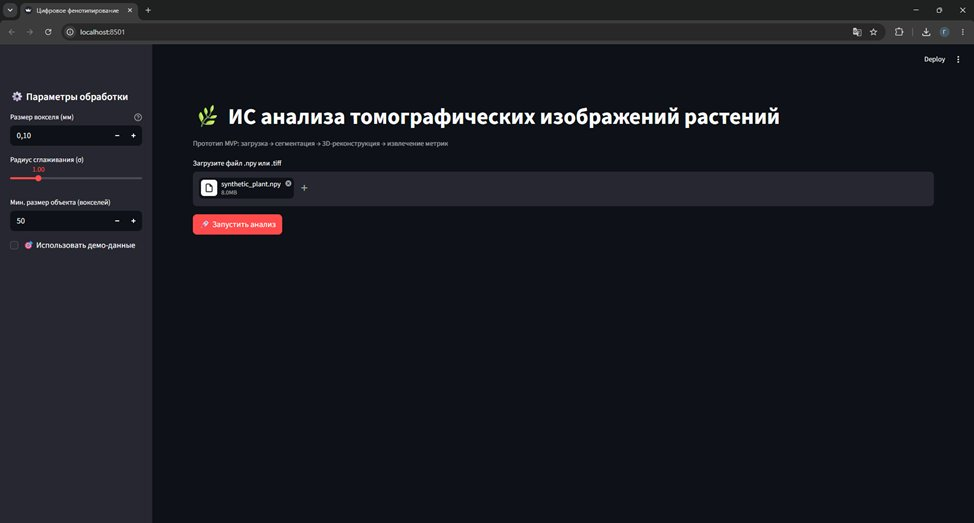
\includegraphics[width=0.95\textwidth]{fig1.png}
  \caption{Интерфейс загрузки сгенерированного файла томограммы}
  \label{fig:interface}
\end{figure}

На рисунке~\ref{fig:interface} представлен главный экран веб-приложения после загрузки тестового файла. В левой части интерфейса расположена боковая панель с параметрами обработки: размер вокселя~--- 0.10~мм, радиус сглаживания ($\sigma$)~--- 1.0, минимальный размер объекта~--- 50~вокселей. В центральной области отображается загруженный файл \texttt{synthetic\_plant.npy} объёмом 8.0~МБ, что соответствует трёхмерному массиву размером $128 \times 128 \times 128$ элементов типа \texttt{float32}.

\subsection{Результаты обработки и анализ фенотипических признаков}

После нажатия кнопки «Запустить анализ» система последовательно выполнила все этапы конвейера: гауссово сглаживание с $\sigma = 1.0$, автоматическую бинаризацию методом Оцу, морфологическую очистку и трёхмерную реконструкцию алгоритмом Marching Cubes. Результаты работы системы представлены на рисунке~\ref{fig:results}.

\begin{figure}[h!]
  \centering
  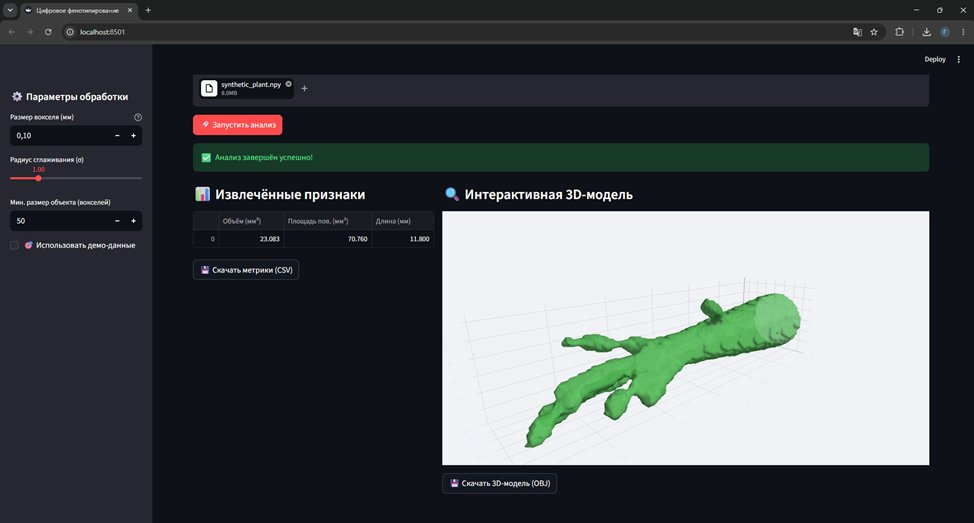
\includegraphics[width=0.95\textwidth]{fig2.png}
  \caption{Результаты работы системы при обработке сгенерированной томограммы: таблица фенотипических признаков и интерактивная 3D-модель реконструированного объекта}
  \label{fig:results}
\end{figure}

В левой части интерфейса отображается таблица извлечённых фенотипических признаков, рассчитанных с учётом физического размера вокселя 0.1~мм. Для реконструированного объекта получены следующие значения:
\begin{itemize}
  \item объём~--- 23.083~мм$^3$, характеризует общую биомассу растительной структуры;
  \item площадь поверхности~--- 70.760~мм$^2$, отражает суммарную площадь всех граней полигональной сетки;
  \item длина~--- 11.800~мм, соответствует максимальной протяжённости объекта по оси роста (ось Z).
\end{itemize}

В правой части интерфейса представлена интерактивная 3D-модель с центральным стеблем конической формы и несколькими боковыми ответвлениями, имитирующими корневые отростки или побеги.

Анализ количественных показателей подтверждает корректность работы алгоритмов. При размере массива 128~вокселей и физическом размере вокселя 0.1~мм максимальная теоретическая протяжённость составляет 12.8~мм, а фактическое значение 11.8~мм указывает, что структура занимает большую часть пространства по оси Z~--- результат согласуется с параметрами генерации.

\newpage

%% ════════════════════ ЗАКЛЮЧЕНИЕ ═════════════════════════════════════════════
\chapter*{ЗАКЛЮЧЕНИЕ}
\addcontentsline{toc}{chapter}{Заключение}

В ходе выполнения курсовой работы была достигнута поставленная цель~--- спроектирован и программно реализован прототип информационной системы для автоматизированного анализа томографических изображений и трёхмерных моделей растений. Последовательно решены все задачи, сформулированные во введении: проведён анализ предметной области и методов неразрушающей визуализации, выполнено сравнительное исследование существующих программных платформ, обоснован выбор клиент-серверной архитектуры и технологического стека, разработаны и интегрированы алгоритмические модули предобработки, сегментации, 3D-реконструкции и расчёта морфометрических признаков, создан интерактивный веб-интерфейс с функцией экспорта результатов.

Практическая реализация системы продемонстрировала корректность работы сквозного конвейера обработки данных. На синтетических томограммах система успешно выполнила автоматическую бинаризацию методом Оцу, морфологическую очистку от артефактов и построение полигональной сетки алгоритмом Marching Cubes. Рассчитанные фенотипические признаки (объём, площадь поверхности, длина) корректно переведены в физические миллиметры, а их значения согласуются с геометрией исходного массива. Интерактивная визуализация в браузере и экспорт результатов в форматы CSV и OBJ подтвердили готовность решения к использованию в учебных и исследовательских задачах.

Практическая значимость работы заключается в создании доступного, воспроизводимого инструмента, снижающего технологический порог входа в цифровое фенотипирование. Система не требует HPC-ресурсов, развёртывается за несколько минут через стандартный менеджер пакетов Python и обеспечивает полную прозрачность алгоритмов. Фиксация параметров обработки и детерминированность вычислений соответствуют принципам открытой науки и стандартам FAIR.

Разработанное решение обладает рядом ограничений учебного формата. Алгоритмическая база опирается на классические методы обработки изображений, что ограничивает точность сегментации при работе с объектами низкого контраста. Производительность оптимизирована для объёмов до $256^3$ вокселей без GPU-ускорения.

Перспективы развития системы связаны с интеграцией нейросетевых моделей сегментации (3D U-Net, nnU-Net), поддержкой мультимодальных входных данных и расширением библиотеки фенотипических метрик (углы ветвления, пористость, топологический скелет). Модульная архитектура допускает масштабирование за счёт подключения внешних алгоритмических пакетов и адаптации под облачные среды.

\newpage

%% ════════════════════ БИБЛИОГРАФИЧЕСКИЙ СПИСОК ═══════════════════════════════
\chapter*{БИБЛИОГРАФИЧЕСКИЙ СПИСОК}
\addcontentsline{toc}{chapter}{Библиографический список}

\begin{enumerate}
  \item Гонсалес,~Р. Цифровая обработка изображений / Р.\,Гонсалес, Р.\,Вудс~; пер. с англ.~--- М.~: Техносфера, 2020.~--- 1072~с.
  \item Лобет,~Ж. Анализ архитектуры корневой системы: от получения изображений к фенотипированию / Ж.\,Лобет, Кс.\,Драй, К.\,Перильё~// Журнал экспериментальной ботаники.~--- 2013.~--- Т.~64, №~15.~--- С.~4773--4785.
  \item Лоренсен,~У.\,Е. Marching Cubes: алгоритм построения трёхмерных поверхностей высокого разрешения / У.\,Е.\,Лоренсен, Х.\,Е.\,Клайн~// Компьютерная графика.~--- 1987.~--- Т.~21, №~4.~--- С.~163--169.
  \item Маккинни,~У. Python для анализа данных / У.\,Маккинни~; пер. с англ.~--- СПб.~: Питер, 2022.~--- 480~с.
  \item Сойфер,~В.\,Н. Компьютерная томография: методы и алгоритмы / В.\,Н.\,Сойфер.~--- М.~: Физматлит, 2019.~--- 384~с.
  \item Документация по библиотеке Plotly: интерактивная визуализация данных~[Электронный ресурс]~// Plotly.~--- URL: \url{https://plotly.com/python/} (дата обращения: 04.05.2026).
  \item Документация по библиотеке scikit-image: обработка изображений на Python~[Электронный ресурс]~// scikit-image.~--- URL: \url{https://scikit-image.org/docs/} (дата обращения: 04.05.2026).
  \item Документация по фреймворку Streamlit: создание интерактивных веб-приложений~[Электронный ресурс]~// Streamlit.~--- URL: \url{https://docs.streamlit.io/} (дата обращения: 04.05.2026).
  \item Принципы FAIR для управления научными данными~[Электронный ресурс]~// GO FAIR.~--- URL: \url{https://www.go-fair.org/fair-principles/} (дата обращения: 04.05.2026).
  \item Репозиторий модуля tifffile: чтение и запись TIFF-файлов~[Электронный ресурс]~// GitHub.~--- URL: \url{https://github.com/cgohlke/tifffile} (дата обращения: 04.05.2026).
\end{enumerate}

\end{document}
